%	PACKAGES AND OTHER DOCUMENT CONFIGURATIONS
%----------------------------------------------------------------------------------------

\documentclass[11pt,fleqn]{book} % Default font size and left-justified equations
\usepackage[export]{adjustbox}
\usepackage[table,xcdraw]{xcolor}

\usepackage[top=3cm,bottom=3cm,left=3.2cm,right=3.2cm,headsep=10pt,letterpaper]{geometry} % Page margins

\usepackage{xcolor} % Required for specifying colors by name
\definecolor{ocre}{RGB}{52,177,201} % Define the orange color used for highlighting throughout the book

% Font Settings
\usepackage{avant} % Use the Avantgarde font for headings
%\usepackage{times} % Use the Times font for headings
\usepackage{mathptmx} % Use the Adobe Times Roman as the default text font together with math symbols from the Sym­bol, Chancery and Com­puter Modern fonts

\usepackage{microtype} % Slightly tweak font spacing for aesthetics
\usepackage[utf8]{inputenc} % Required for including letters with accents
\usepackage[T1]{fontenc} % Use 8-bit encoding that has 256 glyphs
\usepackage{amsmath}
\usepackage{tikz}
\usepackage{mathdots}
\usepackage{yhmath}
\usepackage{cancel}
\usepackage{color}
\usepackage{siunitx}
\usepackage{array}
\usepackage{multirow}
\usepackage{amssymb}
\usepackage{gensymb}
\usepackage{tabularx}
\usepackage{booktabs}
\usetikzlibrary{fadings}
\usepackage[section]{placeins}

% % Bibliography
% \usepackage[style=alphabetic,sorting=nyt,sortcites=true,autopunct=true,babel=hyphen,hyperref=true,abbreviate=false,backref=true,backend=biber]{biblatex}
% \defbibheading{bibempty}{}
\usepackage[style=authoryear-ibid,backend=biber,alphabetic,sorting=nyt,]{biblatex}
\addbibresource{bibliography.bib} % BibTeX bibliography file

\input{structure} % Insert the commands.tex file which contains the majority of the structure behind the template
\let\cleardoublepage\clearpage
\makeatletter
\newcommand{\tocfill}{\cleaders\hbox{$\m@th \mkern\@dotsep mu . \mkern\@dotsep mu$}\hfill}
\makeatother
\newcommand{\abbrlabel}[1]{\makebox[3cm][l]{\textbf{#1}\ \tocfill}}
\newenvironment{abbreviations}{\begin{list}{}{\renewcommand{\makelabel}{\abbrlabel}%
                                              \setlength{\itemsep}{0pt}}}{\end{list}}
\begin{document}
\title{THESIS}

%----------------------------------------------------------------------------------------
%	TITLE PAGE
%----------------------------------------------------------------------------------------

\begingroup
\thispagestyle{empty}
\AddToShipoutPicture*{\put(0,0){\includegraphics[scale=1.2]{Pictures/Cover.png}}} % Image background
\centering
\vspace*{2cm}
\par\normalfont\fontsize{28}{28}\sffamily\selectfont
\textbf{ Valuation Strategies for Utility Energy Battery Storage in the NEM }\\
\vspace*{0.5cm}
{\Large School of Photovoltaic and Renewable Energy Engineering   Faculty of Engineering | 
The University of New South Wales}\par % Book title
\vspace*{0.5cm}
{\LARGE Henry Blumentals }\par % Author name
\endgroup
%-------------------------------------------
%%%%%%%%%%%%%%%%%%%%%%%%%%%%%%%%%
\newpage 

\thispagestyle{empty} 
{\noindent 
\textbf{UNIVERSITY OF NEW SOUTH WALES} \\
Faculty of Engineering \\   
School of Photovoltaics \& Renewable Energy Engineering \\  

\begin{center}
   \LARGE{\textbf{UNDERGRADUATE THESIS}} 
\end{center}

 }
\noindent


\begin{tabbing}
\textbf{Supervisor:} \quad \quad \quad \qquad \= Dr. Anna Bruce,\\ % MODIFY!
\>{\small School of Photovoltaics \& Renewable Energy Engineering} \\ % institute goes here
\>{\small University of New South Wales} \\ % uni. and country
\>{\small Sydney, Australia} \\ % uni. and country
\\
\textbf{Co-supervisor:} 
\> A. Prof. Iain MacGill,\\ % MODIFY!
\>{\small Centre for Energy \& Environmental Markets} \\ % MODIFY!
\>{\small University of New South Wales} \\ % uni. and country
\>{\small Sydney, Australia} \\ % uni. and country
\\
\textbf{Industry  Supervisor:} 
\> Mr. Merrick Underwood \\ % MODIFY!
\>{\small Manager Energy Market Analytics} \\ % MODIFY!
\>{\small Infigen Energy} \\ % uni. and country
\>{\small Sydney, Australia} \\ % uni. and country
\\
\textbf{Project Collaborator:} 
\> Mr. Daniel Tam \\ % MODIFY!
\>{\small Undergraduate Photovoltaic Engineer \& Computer Scientist } \\ % MODIFY!
\>{\small University of New South Wales } \\ % uni. and country
\>{\small Sydney, Australia} \\ % uni. and country
\\
\textbf{Assessors:} 
\> Dr. Anna Bruce, \\ % MODIFY!
\> A. Prof. Iain Macgill.\\ % MODIFY!
\end{tabbing}

\noindent
\textbf{Submitted by:} Henry William Desmond Blumentals, z5059913 \\
\textbf{Submitted on:} X June \Year, Sydney \\ % MODIFY!

\noindent

\begin{tabbing}
\AuthorName \= $\rule{5cm}{0.15mm}$\\
\> \hspace*{1.5cm} {\footnotesize signature} \\ %\hspace*{\fill} 
\end{tabbing}
\hspace{3mm}

\begin{tikzpicture}[remember picture, overlay]
  \node [anchor=north east, inner sep=30pt]  at (current page.north east)
     {\includegraphics[width=30mm]{Pictures/unsw_logo.png}};
\end{tikzpicture}

\clearpage
\thispagestyle{empty}


%--------------------------------------------
\chapter*{Abstract}
\chapter*{Acknowledgements}
\chapter*{Abbreviations}
\par\vspace*{-190\p}
\begin{abbreviations}
\item[NEM] National Electricty Market
\item[BESS] Battery Energy Storage System
\item[PV] Photovoltaic
\item[NEMDE] National Electricity Market Dispatch Engine
\end{abbreviations}
%----------------------------------------------------------------------------------------
%	TABLE OF CONTENTS
%----------------------------------------------------------------------------------------

\chapterimage{neoen.png} % Table of contents heading image

\pagestyle{empty} % No headers

\tableofcontents % Print the table of contents itself

%\cleardoublepage % Forces the first chapter to start on an odd page so it's on the right

\pagestyle{fancy} % Print headers again

%----------------------------------------------------------------------------------------

\chapterimage{GESS-photo.jpg} % Chapter heading image

\chapter{Introduction}
\section{ Utility Battery Energy Storage Overview }

Australia's National Electricity Market (NEM) incorporates around 40,000 km of transmission lines, and supplies about 200 TWh of electricity to approximately 9 million customers each year \parencite{AEMO_NEM}. Currently the NEM is undergoing a rapid transformation in the mix of generation types. A rapid influx in low-cost wind and utility solar photovoltaics (PV) are shifting the merit order of lowest cost generation. Combined with ageing thermal generation, unseen behind the meter PV generation and a rise in demand response, operational challenges pertaining to the stability of the grid are rising. As a reflection of the technical challenges facing the NEM wholesale spot electricity prices have inherently exhibited an increase in volatility, driving the requirement for energy storage and load shifting. Furthermore increases an influx of low inertia generation, combined with misplaced incentives for primary frequency control have produced an increased demand for FCAS Regulation services. 

\url{http://apvi.org.au/solar-research-conference/wp-content/uploads/2018/12/01_DI_Boyle_K_2018.pdf.pdf}

\url{https://www.aemo.com.au/-/media/Files/Electricity/NEM/Initiatives/Emerging-Generation/EGES_Stakeholder_Paper_Final.pdf}

\section{ Thesis Aim and Structure }
Whilst prior work in this field focus' on the base revenue stream of energy-only arbitrage, few have analyzed the value of battery storage systems co-optimising dispatch across multiple services or value streams in accordance with operational strategies.
\chapter{Background and Literature Review}
\section{ The National Electricity Market }
\subsection{ Operation of the Spot Market }
\subsection{ Operation of the Ancillary Service Market }
\subsection{ Pre-dispatch Forecast Process }
Within the NEM, a pre-dispatch process is performed by Australian Energy Market Operator to ensure that market participants have sufficient pricing information to make informed and timely business decisions. In turn, this information provides the market with the information it needs to provide security of supply.  AEMO publishes somewhat limited information during pre-dispatch, however in evaluating battery storage this is vital to ensuring appropriate state of charge for future energy arbitrage opportunities. AEMO processes 2 different pre-dispatch to forecast price, 5 minute and 30 minute.
\subsubsection{P5 Region Solution}
The 5-minute Pre-dispatch cycle runs every 5-minutes to produce a dispatch and pricing schedule to a 5-minute resolution covering the next hour, for a total of twelve periods. It is key to note these prices represent forecasts for 5 minute dispatch prices rather than trading prices. Figure \ref{fig:p5_process_1} shows predicted dispatch price via the P5 Region Solution within the trading interval of 12:30:00pm, on the 1st of January, 2018, in South Australia. 
\begin{figure}[!h]
\centering
\includegraphics[width=0.8\textwidth]{Pictures/Chapter2/P5_Process.png}
\caption{P5 Predispatch Process - South Australia, Trading Interval 01/01/2018 12:30:00 PM}
\label{fig:p5_process_1}
\end{figure}
As seen in Figure \ref{fig:p5_process_1}, the P5 Region solution runs each 5 minutes and accuracy converges as forecast period approaches the dispatch interval. Although the forecast may not appear very accurate, Figure \ref{fig:p5_process_2} shows the P5 Price forecast elapsed for a full 24 hrs, clearly showing price follows the trend set by the forecast. 
\begin{figure}[!h]
\centering
\includegraphics[width=1\textwidth]{Pictures/Chapter2/P5_Process_2.png}
\caption{P5 Pre-dispatch Process - South Australia, 01/01/2018 - 02/01/2018}
\label{fig:p5_process_2}
\end{figure}
To date, no peer-reviewed academic analysis has been performed on the accuracy of the P5 Price forecast. The fundamental justification is most likely the shear size of the data set \textit{(For each year there are over 6 million rows of data for the 5 NEM jurisdictions)}. However, \parencite{AEMCMarch2017} provides insight into the magnitude of P5 Price forecast error by NEM region for the period 1 September 2015 to 8 March 2017, as shown in Figure \ref{fig:p5_aemc}. 
\begin{figure}[!htb]
\centering
\includegraphics[width=1\textwidth]{Pictures/Chapter2/AEMC_P5_Error.PNG}
\caption{AEMC 2017: Magnitude of Forecast Error Varies by Region.}
\label{fig:p5_aemc}
\end{figure}
\parencite{AEMCMarch2017} highlights 3 key elements regarding the P5 price forecast; accuracy improves as dispatch nears, the distribution is relatively symmetric with no apparent bias to overvaluing or under-valuing price and finally South Australia appears to have the greatest price discrepancy in absolute terms, however this is likely to be due to the underlying average price of the state being higher.


\subsubsection{P30 Predispatch Price}

To ensure it reliability of the P30 Predispatch Price forecast, the 48 half hours supply schedules of the following trading day need to be submitted by the generators by 12.30pm on the day before dispatch \parencite{Predispatch}. The expected wholesale electricity prices for the next day are then produced by matching these supply schedules with the demand forecasts, ancillary service requirements, inter-regional and intra-regional limits, in addition to solar and wind energy forecasts. 


\tikzset{every picture/.style={line width=0.75pt}} %set default line width to 0.75pt        

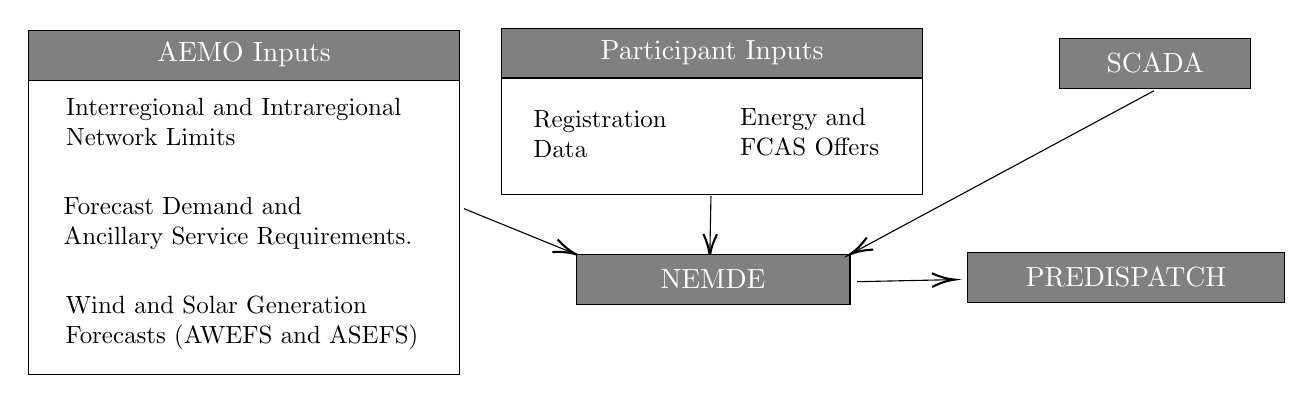
\begin{tikzpicture}[x=0.75pt,y=0.75pt,yscale=-1,xscale=1]
%uncomment if require: \path (0,191.0132598876953); %set diagram left start at 0, and has height of 191.0132598876953

%Straight Lines [id:da9177958313522097] 
\draw    (357.44,91.83) -- (356.91,119.02) ;
\draw [shift={(356.87,121.02)}, rotate = 271.13] [color={rgb, 255:red, 0; green, 0; blue, 0 }  ][line width=0.75]    (10.93,-3.29) .. controls (6.95,-1.4) and (3.31,-0.3) .. (0,0) .. controls (3.31,0.3) and (6.95,1.4) .. (10.93,3.29)   ;

%Straight Lines [id:da12798518797085823] 
\draw    (238.44,97.83) -- (290.59,119.07) ;
\draw [shift={(292.44,119.83)}, rotate = 202.17000000000002] [color={rgb, 255:red, 0; green, 0; blue, 0 }  ][line width=0.75]    (10.93,-3.29) .. controls (6.95,-1.4) and (3.31,-0.3) .. (0,0) .. controls (3.31,0.3) and (6.95,1.4) .. (10.93,3.29)   ;

%Shape: Rectangle [id:dp13477801690658042] 
\draw   (256.5,10.9) -- (459.5,10.9) -- (459.5,90.9) -- (256.5,90.9) -- cycle ;
%Shape: Rectangle [id:dp8582430372753662] 
\draw  [fill={rgb, 255:red, 128; green, 128; blue, 128 }  ,fill opacity=1 ] (256.5,10.9) -- (459.5,10.9) -- (459.5,34.9) -- (256.5,34.9) -- cycle ;
%Shape: Rectangle [id:dp5655505133083187] 
\draw   (28.5,11.9) -- (236.44,11.9) -- (236.44,177.9) -- (28.5,177.9) -- cycle ;
%Shape: Rectangle [id:dp5185219575052318] 
\draw  [fill={rgb, 255:red, 128; green, 128; blue, 128 }  ,fill opacity=1 ] (28.5,11.9) -- (236.44,11.9) -- (236.44,35.9) -- (28.5,35.9) -- cycle ;


%Shape: Rectangle [id:dp11057728244309994] 
\draw  [fill={rgb, 255:red, 128; green, 128; blue, 128 }  ,fill opacity=1 ] (292.44,119.83) -- (424.44,119.83) -- (424.44,143.83) -- (292.44,143.83) -- cycle ;
%Shape: Rectangle [id:dp07113446577922766] 
\draw  [fill={rgb, 255:red, 128; green, 128; blue, 128 }  ,fill opacity=1 ] (525.5,15.9) -- (617.44,15.9) -- (617.44,39.9) -- (525.5,39.9) -- cycle ;

%Straight Lines [id:da9707191163095252] 
\draw    (570.87,41.02) -- (426.2,118.88) ;
\draw [shift={(424.44,119.83)}, rotate = 331.71000000000004] [color={rgb, 255:red, 0; green, 0; blue, 0 }  ][line width=0.75]    (10.93,-3.29) .. controls (6.95,-1.4) and (3.31,-0.3) .. (0,0) .. controls (3.31,0.3) and (6.95,1.4) .. (10.93,3.29)   ;

%Shape: Rectangle [id:dp46501665361769806] 
\draw  [fill={rgb, 255:red, 128; green, 128; blue, 128 }  ,fill opacity=1 ] (480.87,118.83) -- (633.87,118.83) -- (633.87,142.83) -- (480.87,142.83) -- cycle ;
%Straight Lines [id:da4584246014213331] 
\draw    (427.87,133.02) -- (472.87,132.06) ;
\draw [shift={(474.87,132.02)}, rotate = 538.78] [color={rgb, 255:red, 0; green, 0; blue, 0 }  ][line width=0.75]    (10.93,-3.29) .. controls (6.95,-1.4) and (3.31,-0.3) .. (0,0) .. controls (3.31,0.3) and (6.95,1.4) .. (10.93,3.29)   ;


% Text Node
\draw (358,22.9) node [color={rgb, 255:red, 255; green, 255; blue, 255 }  ,opacity=1 ] [align=left] {Participant Inputs};
% Text Node
\draw (304,62) node [scale=0.9] [align=left] {Registration\\Data};
% Text Node
\draw (405,61) node [scale=0.9] [align=left] {Energy and\\FCAS Offers};
% Text Node
\draw (132.47,23.9) node [color={rgb, 255:red, 255; green, 255; blue, 255 }  ,opacity=1 ] [align=left] {AEMO Inputs};
% Text Node
\draw (129.53,105) node [scale=0.9] [align=left] {Forecast Demand and \\Ancillary Service Requirements.};
% Text Node
\draw (127.5,56) node [scale=0.9] [align=left] {Interregional and Intraregional \\Network Limits};
% Text Node
\draw (131.5,153) node [scale=0.9] [align=left] {Wind and Solar Generation \\Forecasts (AWEFS and ASEFS)};
% Text Node
\draw (571.47,27.9) node [color={rgb, 255:red, 255; green, 255; blue, 255 }  ,opacity=1 ] [align=left] {SCADA};
% Text Node
\draw (358.44,131.83) node [color={rgb, 255:red, 255; green, 255; blue, 255 }  ,opacity=1 ] [align=left] {NEMDE};
% Text Node
\draw (557.37,130.83) node [color={rgb, 255:red, 255; green, 255; blue, 255 }  ,opacity=1 ] [align=left] {PREDISPATCH};


\end{tikzpicture}

\caption{AEMO Pre-dispatch Process.}
\label{diagram:predispatch_process}


Those prices are also known as pre-dispatch prices for the next day. The granularity of the predispatch prices are given in 5 minute and 30 minute intervals, the 5 minute and 30 minute predispatch forecasts respectively. The 5-minute predispatch forecast is extends 1 hour whilst the 30-minute predispatch extend until the end of the following trading day with variable time horizon spanning between 28 intervals (14 hrs) up to 79 intervals (39.5 hrs)
\parencite{Predispatch}. \\
Pre-dispatch pricing does vary materially from actual pricing. In March 2017, the AEMC quantitatively highlighted how predispatch accuracy increases as the dispatch period nears.
\begin{table}[!h]
\begin{tabular}{l|c|c|c|}
\cline{2-4}
                                   & \multicolumn{3}{l|}{\cellcolor[HTML]{EFEFEF}\textbf{Percentage of Accurately Predicted High Prices}}                                    \\ \cline{2-4} 
                                   & \multicolumn{1}{l|}{\textit{One hour out}} & \multicolumn{1}{l|}{\textit{Four hours out}} & \multicolumn{1}{l|}{\textit{Ten hours out}} \\ \hline
\multicolumn{1}{|l|}{\textbf{NSW}} & 77\%                                       & 66\%                                         & 59\%                                        \\ \hline
\multicolumn{1}{|l|}{\textbf{QLD}} & 73\%                                       & 61\%                                         & 54\%                                        \\ \hline
\multicolumn{1}{|l|}{\textbf{SA}}  & 61\%                                       & 46\%                                         & 39\%                                        \\ \hline
\multicolumn{1}{|l|}{\textbf{TAS}} & 47\%                                       & 38\%                                         & 33\%                                        \\ \hline
\multicolumn{1}{|l|}{\textbf{VIC}} & 52\%                                       & 52\%                                         & 45\%                                        \\ \hline
\end{tabular}
\end{table}
Justification of tasmania \url{https://www.economicregulator.tas.gov.au/Documents/Energy%20in%20Tasmania%202016-17%20Report.pdf }

\section{ Utility Battery Energy Storage Dispatch Models }
\subsection{ Energy Arbitrage }
\subsection{ Energy Arbitrage with Imperfect Foresight }
\subsection{ Energy Arbitrage with Co-optimised with FCAS Participation }
\subsection{ Performance of Existing Utility Battery Energy Storage Plants in the NEM }
\subsubsection{ Hornsdale Power Reserve }
\subsubsection{ Gannawarra Energy Storage System }
\subsubsection{ Lake Bonney Precinct Battery Energy Storage System }
\section{ NEM Changing Generation Mix  }
\subsection{ Overview }
\subsection{ Modelling Techniques }
\section{ Policy and Investment Supporting Utility Storage   }
\subsection{ Australian Context }
\subsection{ Examples Abroad }

\section*{Citation examples}
\begin{enumerate}
\item A citation command in parentheses: \parencite{Smith:2012qr}.
\item A citation command for use in the flow of text: As \textcite{Smith:2013jd} said \dots
\item A citation command which automatically switches style depending on location and the option setting in the package declaration (see line 12 in the LaTeX source code). In this case, it produces a citation in parentheses: \autocite{Other:2014ab}.
\end{enumerate}
\chapter{ Utility Battery Energy Storage - Energy Arbitrage Only}
In the most elementary form, energy arbitrage entails charging when the wholesale spot price is low, and discharging when the wholesale price is high. Whilst conceptually simple, the purchase price of a battery is high, and there are physical limitations on charge/discharge and the frequency of high spot prices is relatively infrequent.
\section{ Algorithm and Software Selection }
\parencite{McConnell} used COIN-OR Linear Program solver to find the optimal dispatch for a battery performing energy arbitrage. Linear programming is one of the most common optimisation techniques. Leonard Kantrovich was awarded the 1975 Nobel Price in Economics for the optimal allocation of resources using linear programming \parencite{PythonPulp}. Examples of problems that can be solved by linear programming include:
\begin{itemize}
    \item Scheduling – Rota or Factory scheduling to meet production/workload demands at lowest cost
    \item Resourcing Problems – How best to allocate resources to maximise profits
    \item Sudoku
\end{itemize}
PuLP is a suitable tool to perform LP in this thesis for the following reasons: 
\begin{itemize}
    \item Library for Python which is a highly supported coding language with an emphasis on rapid development, clarity of code and a simple object model. 
    \item PuLP works entirely within the syntax of Python and represents optimisation problems and decision variables in  a way that is very similar to the original mathematical expression. 
    \item PuLP is available under a permissive open-source license that encourages and facilitates the use of PuLP inside other projects that need linear optimisation capabilities.
\end{itemize}
\section{ Methodology }
The following algorithm represents the methodology for optimising energy arbitrate in a deterministic model with perfect foresight of energy prices over the optimisation window.
\begin{align*}
  \max \sum_{i=0}^T \left(x^{(i)}_c + x^{(i)}_d \right) p^{(i)} \times \left( \frac{l}{60} \right)
\end{align*}
Subject to the constraints:
\begin{alignat} {2}
    -P_{max} &\leq x^{(i)}_c \leq 0  &&\forall i \in [0,T]\\
    0 &\leq x^{(i)}_d \leq P_{max}  &&\forall i \in [0,T]\\
    0 &\leq E^{(i)} \leq E_{max} &&\forall i \in [0,T] \\
    E^{(0)} &= E_{\text{init}} - \left(x^{(0)}_c \eta_c + x^{(0)}_d \frac{1}{\eta_d} \right) \frac{l}{60} && \\
    E^{(i)} &= E^{(i-1)} - \left(x^{(i)}_c \eta_c + x^{(i)}_d \frac{1}{\eta_d} \right) \frac{l}{60} \hspace{1cm} &&\forall i \in [1,T] 
\end{alignat}
Where,
{\renewcommand{\arraystretch}{2}}
\begin{center}
    \begin{tabular}{p{0.8cm} p{5.5cm} p{0.8cm} p{5.5cm}}
    \textbf{Constants} & & \textbf{Variables} & \\
    $P_{max}$ & Power Capacity of BESS (MW) & $x^{(i)}_c$ & Charge power at time $i$ (MW)   \\ 
    $E_{max}$ & Storage Capacity of BESS (MWh) & $x^{(i)}_c$&  Discharge power at time $i$ (MW)  \\
    $E_{\text{init}}$ & Initial Storage Level of BESS (MWh)& $E^{(i)}$ &Storage level at time $i$ (MWh)\\
    $l$ & length of time interval in minutes & & \\
    $\eta_c$ & Charge efficiency (\%) & &\\
    $\eta_d$ & Discharge efficiency (\%) & &\\
    $p^{(i)}$ &  Energy price at time $i$ (\$/MWh) & &\\
    $T$ &  Total number of time intervals & &\\
    \end{tabular}
\end{center}
To implement this algorithm, the following methodology was undertaken;
\begin{enumerate}
    \item Configure a Python 3.7 environment.
    \item Import price data via NEMOSIS:  \url{https://github.com/UNSW-CEEM/NEMOSIS}. NEMOSIS is a simple tool for creating datasets using publicly available information about the Australian National Electricity Market (NEM).
    \item Create a battery object.
    \item PuLP python optimisation problem formulation;
    \begin{enumerate}
        \item Identify the Decision Variables
        \item Formulate the Objective Function using the decision variables
        \item Formulate the Constraints
    \end{enumerate}
\end{enumerate}
It is crucial to note that the energy arbitrage only model assumes the battery is a price-taker,and has perfect foresight of price.
\section{ Analysis }
\subsection{ Method Validation }
As shown in Figure \ref{fig:simple_output}, the dispatch logic charging during low prices, and discharging during high prices is effective. Note in Figure \ref{fig:simple_output} a single trip efficiency of 90\% or round trip efficiency of 81\% is implemented. This is a conservative measure, with Tesla stating their Power Pack round trip efficiency is 88\% \url{https://www.tesla.com/en_AU/powerpack}. 
\begin{figure}[H]
    \centering
    \makebox[\textwidth][c]{    \includegraphics[width=1.1\textwidth]{"Pictures/Chapter3/battery_plot".pdf}}
    \caption{BESS Output - 2018-01-01}
    \label{fig:simple_output}
\end{figure}
In order to validate the model, \parencite{Wang} provides energy arbitrage revenues for a 1MW ESS with capacity between 1-8MWh, using NEM price data for years 2010-2013 with perfect foresight. The model assumes 90\% single trip efficiency. The findings are summarised in Figure \ref{fig:wang_ea}. 
\begin{figure}[H]
    \centering
    \includegraphics{Pictures/Chapter3/wang_ea.PNG}
    \caption{Energy Arbitrage - Geographic and Temporal Comparison (Wang 2016)}
    \label{fig:wang_ea}
\end{figure}
Below, Figure \ref{fig:wang_ea_comparion} is the implementation of the python model replicating Wang's results. 
\begin{figure}[H]
    \centering
    \makebox[\textwidth][c]{    \includegraphics[width=1\textwidth]{"Pictures/Chapter3/ae_wang_comparison".pdf}}
    \caption{Energy arbitrage annual revenue for a 1 MW / 1 MWh BESS by region 2010 - 2013}
    \label{fig:wang_ea_comparion}
\end{figure}
\begin{wrapfigure}{r}{0.6\textwidth}
    \begin{center}
        \includegraphics[width=0.4\textwidth]{Pictures/Chapter3/energy_vol.png}
    \end{center}
    
    \caption{National Electricity Market Demand Volatility \parencite{McConnell}}
    \label{fig:demand_volatility}
\end{wrapfigure}
Given Figures \ref{fig:wang_ea} and \ref{fig:wang_ea_comparion} exhibit identical characteristics, this validates the energy only model. This preliminary example also highlights a number of key findings;
\begin{enumerate}
    \item NSW is on average the worst performing state for energy arbitrage.
    \item SA is consistently a high performer relative to other states.
    \item Large discrepancies can occur year-to-year.
    \item Additional storage which increases the cost of a battery proportionally offers diminishing returns for all example. This indicates that short price spikes generally drive revenue, rather than sustained high prices periods. 
\end{enumerate}
Figure \ref{fig:demand_volatility} provided by \textcite{McConnell} highlights the daily variation in demand for each NEM jurisdiction (excl. TAS). Demand volatility which inherently drives price volatility, generally reflects economic and climatic factors. As shown in Figure \ref{fig:demand_volatility}, South Australia has the highest ratio of maximum to minimum daily demand.  
\subsection{ Dependency on Price Dynamics }
Figure \ref{fig:revenue_duration} displays a revenue duration curve of a 1MW/1MWh BESS with 90\% round-trip efficiency from FY 2010 - 2017. The logarithmic scale clearly indicates that less than 10\% of the time, a very significant proportion of revenue is raised from infrequent, high price events. Figure \ref{fig:revenue_duration} also demonstrates an increase in overall BESS revenue - beyond 2013 (not reflected in Figure \ref{fig:wang_ea_comparion}). 
\begin{figure}[H]
    \centering
    \makebox[\textwidth][c]{    \includegraphics[width=1\textwidth]{"Pictures/Chapter3/Revenue Duration Curve for FY10 - FY17".pdf}}
    \caption{Revenue Duration Curve for FY10 - FY17}
    \label{fig:revenue_duration}
\end{figure}
\begin{wrapfigure}{r}{0.6\textwidth}
    \begin{center}
        \includegraphics[width=0.6\textwidth]{Pictures/Chapter3/mcconnell_revenue_duration.png}
    \end{center}
    \caption{BESS Revenue Duration Curve (McConnell 2014)}
    \label{fig:mcconnell_rev_duration}
\end{wrapfigure}
 Again, the work of McConnell reinforces this notion in Figure  \ref{fig:mcconnell_rev_duration}. Overall, this phenomenon is expected due to the high Market Clearing Price (MCP) of the NEM at \$14,500.  A high MCP is an essential ingredient to electricity market design. In case of scarcity situations and extreme market fundamentals – such as a heat wave in South Australia, prices may sore to \$14,500/MWh for a number of intervals. This might sound extreme, but have been observed from time to time in the past few years. Such economically justified scarcity prices have a negligible impact on the average price of
electricity for end consumers – however, they are vital for the profitability of flexible power plants \parencite{scarcity_pricing}. 
\subsection{ Seasonal Impact }
Figure \ref{fig:mcconnell_heatmap} illustrates the average optimal operating regime for different hours of the day and different days of the year in South Australia. As expected, the dispatch follows the seasonal price and demand patterns characterised by a bi-modal peak in winter and an afternoon peak in summer.
\begin{figure}[H]
    \centering
    \includegraphics[width=0.6\textwidth]{Pictures/Chapter3/mcconnel_heatmap.png}
    \caption{Optimal BESS operation characteristics, for winter and summer months of the year. (McConnell, 2015)}
    \label{fig:mcconnell_heatmap}
\end{figure}
Figure \ref{fig:heatmap} extends the analysis of McConnell, demonstrating the impact that storage capacity has on operating characteristics. The contrast in both sides of the subplot is that 1 Hour storage often has idle times (cream colour) whilst 8 Hours of storage is constantly either charging or discharging.
\begin{figure}[H]
    \centering
    \makebox[\textwidth][c]{    \includegraphics[width=1\textwidth]{"Pictures/Chapter3/South Australia - 2017".pdf}}
    \caption{Optimal BESS operation characteristics, for winter and summer months of the year, varying storage capacity.}
    \label{fig:heatmap}
\end{figure}
\subsection{ Impact of Throughput Constraints }
Below Figure \ref{fig:throughput_limit} shows the impact of applying a 365 cycles per annum throughput limit on a battery energy storage system. As shown, for both region and storage capacity - throughput limitations typically don't hinder arbitrage revenues significantly. 
\begin{figure}[H]
    \centering
    \makebox[\textwidth][c]{    \includegraphics[width=1\textwidth]{"Pictures/Chapter3/Impact of Throughput on Annual Revenue_ 1 MW Battery".pdf}}
    \caption{Impact of Throughput on Annual Revenue: 1 MW Battery}
    \label{fig:throughput_limit}
\end{figure}
\subsection{ Recent Trends and Driving Factors for Energy Arbitrage Revenue }
Figure \ref{fig:wang_plot_full} extends Figure \ref{fig:wang_ea_comparion} and shows the energy arbitrage revenue with perfect foresight, for a 1MW BESS including the calendar years (15,16,17,18). 
\begin{figure}[H]
    \centering
    \makebox[\textwidth][c]{    \includegraphics[width=1\textwidth]{"Pictures/Chapter3/Energy Arbitrage - Geographic and Temporal Comparison".pdf}}
    \caption{Energy arbitrage annual revenue for a 1 MW / 1 MWh BESS by region 2010 - 2018}
    \label{fig:wang_plot_full}
\end{figure}
\begin{wrapfigure}{r}{0.6\textwidth}
    \begin{center}
        \includegraphics[width=0.6\textwidth]{Pictures/Chapter3/generator_gaming.png}
    \end{center}
    \caption{Increase in total value traded in the NEM from bidding games, \$ millions (Grattan Institute, 2018)}
    \label{fig:generator_gaming}
\end{wrapfigure}
Figure \ref{fig:wang_plot_full} highlights a number of key findings. Firstly. Since 2014, the arbitrage value of battery energy storage has clearly increased. 
\newline
Secondly, 2016 witnessed the highest revenues,  especially in South Australia.  \parencite{2016_prices} described the driving force behind the high volatility in 2016 attributable to the removal of the Northern Power Station. \textcite{2016_prices} also highlights a combination of high winter demand, low wind generation, planned upgrades to the Heywood interconnector, in combination with low levels of gas fired generation that coincided with high gas prices all contributed to high volatility.
\newline
Thirdly, Queensland in 2017 exhibited the highest revenue across the states. \parencite{grattan} attributes such volatility in 2017 to Queensland’s government-owned generation companies, Stanwell Corporation and CS Energy, (who provided 71 per cent of all electricity in Queensland in 2016–17), and reported record profitability; 30.4 and 58.9 per cent ROE, respectively. As shown in Figure \ref{fig:generator_gaming}, the value of bidding games have drastically increased in Queensland over the past decade. Gaming in the NEM can cause extreme price fluctuations, as shown in Figure \ref{fig:generator_gaming_1}. Figure \ref{fig:generator_gaming_1} highlights seven dispatch intervals that were near the market price cap of \$14,200/MWh, while most dispatch intervals were around \$100/MWh. In June 2017, the Queensland Government announced
the Powering Queensland Plan, which included a directive to Stanwell Corporation to \textit{“undertake strategies to place downward pressure on
wholesale prices"}. This aligns with Figure \ref{fig:wang_plot_full} as QLD 2018 revenues drop below NSW for the first time since 2011.
\begin{figure}
    \centering
    \includegraphics[width=0.6\textwidth]{Pictures/Chapter3/generator_gaming_2.png}
    \caption{5-minute dispatch interval
price by state for 12 January 2017 (Wood, 2018)}
    \label{fig:generator_gaming_1}
\end{figure}
\chapter{ Energy Arbitrage, Imperfect Foresight }
\section{ AEMO Predispatch Forecast Accuracy }
\subsection{ P30 Predispatch Forecast  }
\subsection{ P5 Predispatch Forecast  }
\section{ Methodology }
\section{ Analysis }
\begin{center}
\begin{figure}[!h]
  \caption{FY 2014 - BESS Arbitrage Revenue, Perfect vs. Imperfect Foresight - McConnell (2015)}
  \centering
\includegraphics[width=0.8\textwidth]{Pictures/Chapter4/2014_Comp_McCon.png}
\end{figure}
\begin{figure}[!h]
  \caption{FY 2014 - BESS Arbitrage Revenue, Perfect vs. Imperfect Foresight - Blumentals, Tam (2019) }
  \centering
\includegraphics[width=0.8\textwidth]{Pictures/Chapter4/2014_Comp.png}
\end{figure}
\end{center}
\subsection{ Impact of NEM Region, Period and Storage Capacity }
\foreach \x in {NSW,SA,VIC, QLD, TAS}
{ \begin{figure}[!h]
  \caption{\x \; BESS Arbitrage Revenue, Perfect vs. Imperfect Foresight }
  \centering
  \hspace*{-2cm}
\includegraphics[width=1.2\textwidth]{Pictures/Chapter4/\x_Comp.png}
\end{figure}
}

\foreach \x in {NSW,SA,VIC, QLD, TAS}
{ \begin{figure}[!h]
  \caption{\x \; Predispatch Forecast Error }
  \centering
  \hspace*{-2cm}
\includegraphics[width=1.2\textwidth]{Pictures/Chapter4/\x_Predispatch_Accuracy.png}
\end{figure}
}

\subsection{ Impact of P30 Predispatch Accuracy }
\subsection{ Impact of Dynamic Throughput Constraints }
\subsection{ Impact of Applying Bidding Characteristics }
\chapter{Co-optimised Energy Arbitrage with Regulation Participation}
\section{ Methodology }
\section{ Analysis }
\subsection{  Impact of Energy Throughput During Regulation Participation }
\subsection{ Impact of  Contingency Revenue }
\subsection{ Validation of Existing Asset Performance  }
\textbf{Method}
\begin{itemize}
  \item Run Co-optimised Regulation and Energy Arbitrage Model Over Historic Data
  \item Run Energy Only with Perfect Foresight over historic data
  \item Run Energy Only Imperfect Foresight Model with Bid Model over Historic Data
     \begin{itemize}
     \item Adjust Bid Model to Ensure Reasonable annual energy throughput. 
   \end{itemize}
  \item Find the Discount Factor i.e 40\% of Imperfect Foresight with Bid Model and Throughput Constraints and Apply to Co-optimised Revenue to Approximate Historic Asset Performance. 
  \item Compare and Justify Differences
\end{itemize}
\chapter{ Performance under a Changing Generation Mix}
\section{ Methodology }
\section{ Analysis }
\subsection{ Impact of Additional Storage }

\chapter{ Performance under a Changing Generation Mix}
\section{ Methodology }
\begin{figure}[H]
    \centering
    \makebox[\textwidth][c]{    \includegraphics[width=\textwidth]{"Pictures/Chapter6/diurnal_profile_low_solar".pdf}}
    \caption{2020 Re-based SA Price Diurnal Profiles with 500MW MW additional solar PV.}
    \label{fig:bess_w_low_solar}
\end{figure}
\begin{figure}[H]
    \centering
    \makebox[\textwidth][c]{    \includegraphics[width=\textwidth]{"Pictures/Chapter6/diurnal_profile_high_solar".pdf}}
    \caption{2020 Re-based SA Price Diurnal Profiles with 1000 MW additional solar PV.}
    \label{fig:bess_w_high_solar}
\end{figure}
\section{ Analysis }
\begin{figure}[H]
    \centering
    \makebox[\textwidth][c]{    \includegraphics[width=\textwidth]{"Pictures/Chapter6/bess_w_solar".pdf}}
    \caption{30MW/119MW BESS energy arbitrage revenue under 2020 BAU, low and high solar.}
    \label{fig:bess_w_solar}
\end{figure}


\chapter*{References}
\printbibliography[heading=none]

 
\end{document}